\subsection{Graph Coloring}
Given a graph $G = (V, E)$, a valid coloring is an assignment of colors to the vertices, so that if $u$ and $v$ are adjacent then they get different colors.

Graph 3-coloring decision problem (3-COL):
\begin{itemize}
	\item Instance: graph $G$.
	\item Question: Is there a valid coloring of $G$ with 3 colors?
\end{itemize}

Clearly in NP. The certificate is just the colors assigned to each vertex. An algorithm can check in polynomial time that only 3 colors are being used, and that adjacent vertices have different colors.

\subsection{3-COL is NP-complete}
We now have a choice of which NP-complete problem to reduce to 3-COL. It turns of 3-SAT is still the right one!

Let $\varphi = \wedge_{i=1}^m C_i$ where $C_i$, the $i$-th clause, is equal to $(l_1^i \vee l_2^i \vee l_3^i)$. The reduction $f$ transforms $\varphi$ into a graph $G$ such that $\varphi$ is satisfiable if and only if $f(\varphi)$ is 3-colorable.

Recall that to make $\varphi$ true, we must make at least 1 literal true in each clause. Then we may consider:
\begin{itemize}
	\item How do we relate the truth values of variables to colors in a graph?
	\item How do we ensure that if $x$ is assigned to TRUE, then $\bar{x}$ is assigned to FALSE (and vice versa)?
	\item How do we translate a clause being satisifiable to some portion of the graph being colorable?
\end{itemize}
\subsubsection{Relating Truth Values To Colors}
Add a triangle on 3 vertices $a$, $b$ and $c$ (called the ``reference triangle'') to the graph. In any valid coloring, $a$, $b$ and $c$ must be colored using all 3 colors. Arbitrarily designate $a$'s color TRUE, $b$'s color FALSE, and $c$'s color to be RED. Make nodes for each pair of literals $x_i$ and $\bar{x_i}$. 

How do we ensure that exactly one of these will be colored TRUE, the other colored FALSE, and neither colored RED? The Answer is simple, make $x_i$ and $\bar{x_i}$ adjacent to each other and to $c$.

\begin{figure}[H]
	\centering
	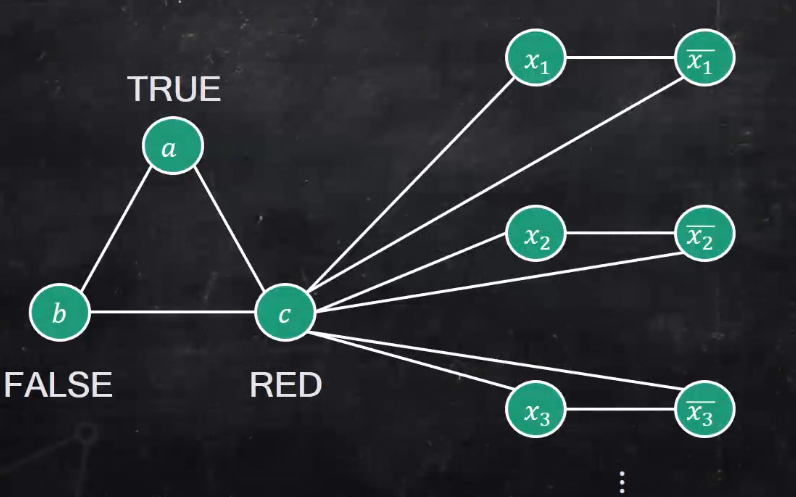
\includegraphics[width=0.5\textwidth]{fig/3-col.png}
\end{figure}

Now let's add more constrain on the graph for the clauses. Consider a clause like $(x \vee y \vee z)$. We already have nodes for $x$, $y$ and $z$ (each of which is forced to be colored TRUE or FALSE). We connect them by a nice ``OR'' gadget as follow:

\begin{figure}[H]
	\centering
	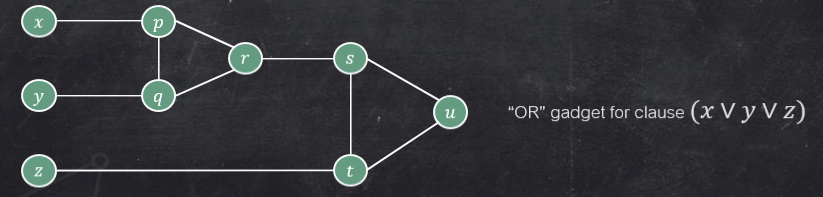
\includegraphics[width=0.7\textwidth]{fig/3-col-or-gadget.png}
\end{figure}

It can be checked the if at least one of $x$, $y$ and $z$ is colored TRUE, then $u$ can be colored TRUE. Otherwise, if all 3 of $x$, $y$ and $z$ are colored FALSE, $u$ must be colored FALSE.

For each clause, add this gadget to the graph using distinct nodes, except for the literal nodes shared between all clauses. Note that, each gadget has its own $p$, $q$, $r$, $s$ $t$ and $u$. For example,

\begin{figure}[H]
	\centering
	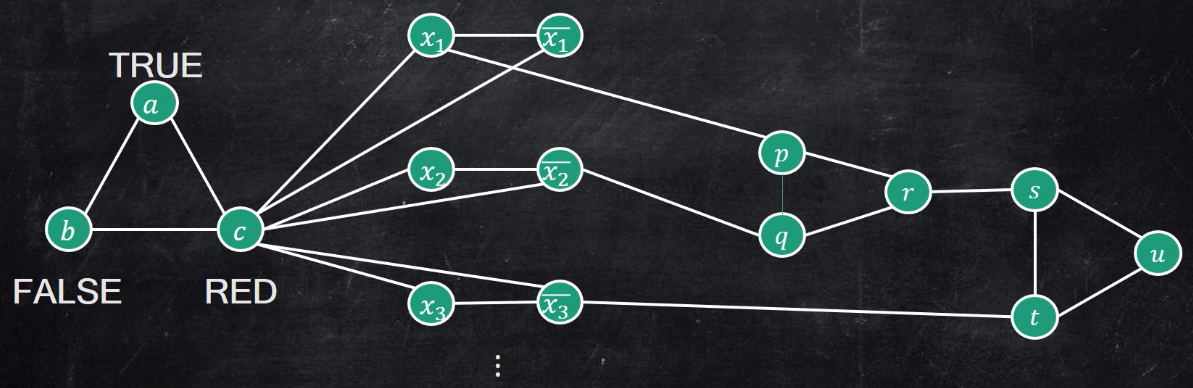
\includegraphics[width=0.7\textwidth]{fig/3-col-or-gadget-in-graph.png}
\end{figure}

To finish off the construction, connect the node at the tip of each clause gadget (labeled $u$ in our example figure) to node $b$ and $c$ in the reference triangle, whose colors are FALSE and RED respectively. In order for this graph to be 3-colorable, we are forced to color the node at the tip of each clause gadget ($u$) TRUE. This is only possible if one of the literals input to the clause is TRUE.

\subsubsection{Proving Correctness}
Our intuition built up in constructing the reduction translates easily into a correctness proof.

Suppose we  start with a YES-instance, $\varphi$ of 3-SAT, use a satisfying assignment to decide which literal in each pair to color ``True'' (the color of $a$ in the reference triangle) and which one to color ``FALSE'' (the color of $b$). Now complete the coloring-assignment by coloring each clause gadget so that node $u$ at the tip of each gadget has color TRUE. This shows we have create a YES-instance of 3-COL!

Conversely, if the reduction created a YES-instance of 3-COL, then look at a valid coloring and treat as true all the literals colored the same as $a$. This sets at least one literal true in each clause. Otherwise we wouldn't have been able to color the clause gadget.

\subsubsection{Wrapping Up}
Reduction is easily computed in polynomial time. When constructing a reduction, remember these points:
\begin{itemize}
	\item Reduce from known NP-complete problem to problem you want to prove NP-complete. Getting the direction of the reduction wrong is a common but serious error.
	\item Do not try to ``solve'' either problem. It's unlikely that you can do it correctly and efficiently.
	\item Instead, do the reduction without knowing whether the instance you are transforming is a YES-instance or a NO-instance.
\end{itemize}

\subsubsection{Motivation}
Graph coloring is an important problem.

``Interference graphs'' are graphs where every node is a task, person, or entity, and edges denote tasks that interfere with one another or people who do not get along. A valid coloring is a way of assigning ``slots'' to these entities so that interfering entities get different slots. Example applications include: compilers allocating variables to registers, allocating frequencies to radio stations, people to tasks, etc.

The bad news is that we have just shown that finding the best solution is unlikely to be efficient.  We must resort to heuristics, or restrict the type of graph. We have already seen one example of the latter: activity selection.

































